\section{Description des différentes spécifications définies en travaux dirigés}

\subsection*{Objectif}

Les spécifications ont pour objectif de définir le comportement attendu du système, autrement dit, ce qui doit être réalisé en réponse au cahier des charges. Elles constituent l’expression formelle des besoins fonctionnels, en se plaçant du point de vue de l’environnement du système — c’est-à-dire de tout ce qui est externe au circuit mais interagit avec lui.
\newline

La phase de spécification représente la première étape de la conception d’un circuit. Elle adopte une approche boîte noire : on s’intéresse uniquement à ce que le système doit faire, sans se préoccuper des solutions techniques internes ni du comment il fonctionnera. Les spécifications sont donc indépendantes de la technologie utilisée.
\newline

Au départ, nous avions pour indication de créer un bloc capable de communiquer à la fois avec le système de trame LIN et avec le microcontrôleur. Afin de simplifier notre étude et nos spécifications, nous avons choisi de diviser le système en deux parties : la réception de trame, qui se chargera de gérer la réception des données octet par octet, et un autre bloc dédié à la communication avec le microcontrôleur.
\newline

% Feuille 1 NOLAN 
\begin{figure}[H]
   \centering
   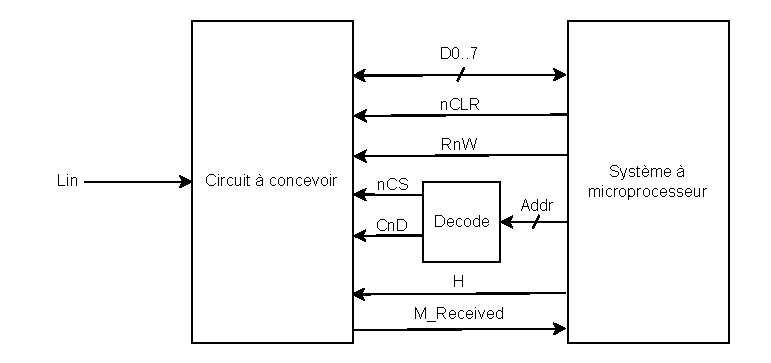
\includegraphics[width=0.8\linewidth]{images/CDC/Schema_cdc_final.pdf}
   \caption{Interface microprocesseur associée au circuit à concevoir}
   \label{fig:placeholder}
\end{figure}
    

\subsection{Interface Microprocesseur}

D'après les données du cahier des charges, nous pouvons définir tous les signaux nécessaires pour le système interface microprocesseur : 

\begin{center}
\renewcommand{\arraystretch}{1.2} % espace vertical
\small % pour uniformiser la taille du texte
\begin{tabularx}{\textwidth}{|c||c|c|X|}
    \hline			
    \textbf{Signaux} & \textbf{Mode} & \textbf{Type} & \textbf{Description}  \\ \hline 
    D07 & INOUT & \texttt{STD\_LOGIC\_VECTOR(7 DOWNTO 0)} & Bus de données \\
    nCS & IN & \texttt{STD\_LOGIC} & Chip Select \\
    RnW & IN & \texttt{STD\_LOGIC} & Operation Lecture / Ecriture \\
    CnD & IN & \texttt{STD\_LOGIC} & Operation Contrôle / Données \\
    nCLR & IN & \texttt{STD\_LOGIC} & Réinitialisation \\
    M\_Received & OUT & \texttt{STD\_LOGIC} & Fin de réception de la trame \\
    H & IN & \texttt{STD\_LOGIC} & Horloge \\
    \hline  
\end{tabularx}
\end{center}


\subsection{Reception Trame}

D'après les données du cahier des charges, nous pouvons définir tous les signaux nécessaires pour le système interface microprocesseur : 

\begin{center}
\renewcommand{\arraystretch}{1.2} % pour un peu plus d'espace vertical
\small % pour uniformiser la taille du texte
\begin{tabularx}{\textwidth}{|c||c|c|X|}
    \hline			
    \textbf{Signaux} & \textbf{Mode} & \textbf{Type} & \textbf{Description}  \\ \hline 
    LIN & IN & \texttt{STD\_LOGIC} & Reception de la trame LIN \\
    \hline  
\end{tabularx}
\end{center}

\subsection{FIFO}

Pour le moment, nous savons qu’il s’agit d’un registre de stockage fonctionnant en mode FIFO, destiné à mémoriser les données de réception d’une trame LIN : 

\begin{center}
\renewcommand{\arraystretch}{1.2} % pour un peu plus d'espace vertical
\small % pour uniformiser la taille du texte
\begin{tabularx}{\textwidth}{|c||c|c|X|}
    \hline
    \textbf{Signaux} & \textbf{Mode} & \textbf{Type} & \textbf{Description} \\ \hline
    OctetRecu & IN & \texttt{STD\_LOGIC\_VECTOR(7 DOWNTO 0)} & Signal Entrée \\
    OctetLu & OUT & \texttt{STD\_LOGIC\_VECTOR(7 DOWNTO 0)} & Signal Sortie \\
    \hline
\end{tabularx}
\end{center}

\subsection{ETAT}

Ce registre peut être considéré comme le registre de log de la trame. Grâce au cahier des charges, nous connaissons précisément ses fonctionnalités :

\begin{center}
\renewcommand{\arraystretch}{1.2} % espace vertical
\small % pour uniformiser la taille du texte
\begin{tabularx}{\textwidth}{|c||c|c|X|}
    \hline			
    \textbf{Signaux} & \textbf{Mode} & \textbf{Type} & \textbf{Description}  \\ \hline 
    Erreur\_Start & IN & \texttt{STD\_LOGIC} & Bit d'erreur de Start \\
    Erreur\_Stop & IN & \texttt{STD\_LOGIC} & Bit d'erreur de Stop \\
    Erreur\_SynchroBreak & IN & \texttt{STD\_LOGIC} & Bit d'erreur de Synchro Break \\
    NbOctetReceived & IN & \texttt{STD\_LOGIC\_VECTOR(3 DOWNTO 0)} & Nombre d'octets reçus \\
    MessageReceived\_SET & IN & \texttt{STD\_LOGIC} & Indicateur de trame reçue \\
    EtatLu & OUT & \texttt{STD\_LOGIC\_VECTOR(7 DOWNTO 0)} & Octet d'information de la trame \\
    \hline  
\end{tabularx}
\end{center}
